\documentclass[11pt,letterpaper]{article}
\usepackage[latin1]{inputenc}
\usepackage{amsmath}
\usepackage{amsfonts}
\usepackage{amssymb}
\usepackage{graphicx}
\usepackage{capt-of}

\setlength{\parskip}{1pc}
\setlength{\parindent}{0pt}
\setlength{\topmargin}{-3pc}
\setlength{\textheight}{9.0in}
\setlength{\oddsidemargin}{0pc}
\setlength{\evensidemargin}{0pc}
\setlength{\textwidth}{6.5in}

\title{6.170 Assignment 4 Documentation}
\author{Dina Betser}


\begin{document}
\maketitle

\section{Models}
\subsection{Object Models}
The object model for the problem domain is included in the figure below. The problem domain object model demonstrates the system that must be built. 

The top-level object is a \texttt{Game}, which includes the concepts of \texttt{Player}s, a \texttt{Board}, a play \texttt{Mode}, a \texttt{GameStateHistory} for undo/redoing moves, and \texttt{GameStats} to store things like the number of boxes allocated to each player.
\begin{center}
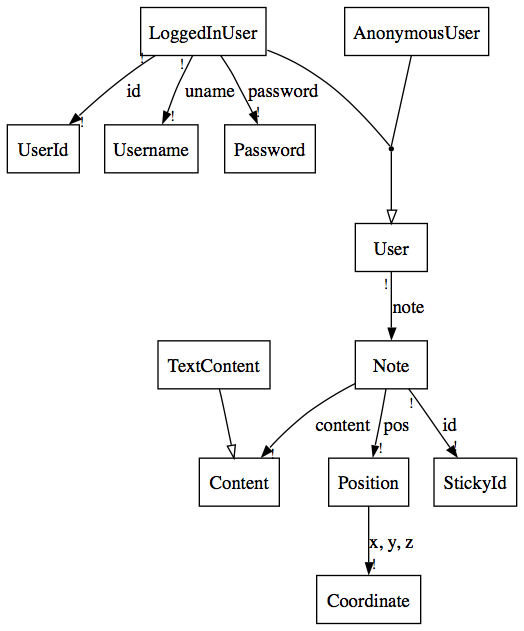
\includegraphics[width=10.5in, angle=90]{dot/obmod.png}
\label{fig:ob1} 
\end{center}

\subsection{State Machines}
The following state machine describes how the state of the application changes as game play progresses.
\begin{center}
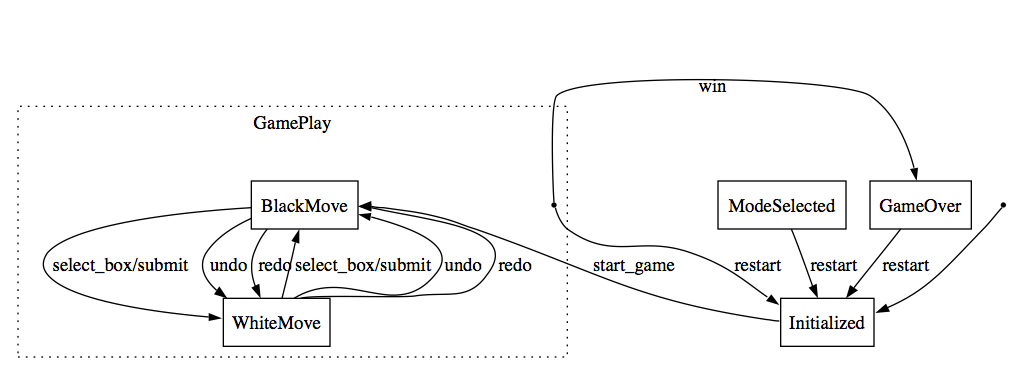
\includegraphics[width=7in]{dot/statediag.png}
\label{fig:sm1} 
\end{center}

\section{Design Notes}
\subsection{Key Challenges}
\begin{itemize}
\item One of the main challenges of this assignment was implementing the gameplay logic. Using online resources, I was able to get an idea of how the markers are reversed in accordance with the game rules.
\item Organizing the code to ensure that changes to the UI were not made directly from the \texttt{Game} ADT, which served as the bulk of the model in the MVC format. Callbacks were crucial in achieving this result. Doing so supported Separation of concerns, and helped implement a View and Model that remained linked by a Controller entity.
\item Implementing undo/redo. This was done using a stack that stored \texttt{GameStateData} objects, each of which encapsulates the state of the board and the statistics of the game such as the current player and the number of boxes belonging to the black player, the white player, and still unallocated. 
\item How to switch players with human vs. human play. Because I based my code structure on tictactoe.js, the code originally supported a given ``round'' with every box click, with both human and computer player. It required a lot of manipulation of state to allow for two humans to play each other instead of automatically playing for the computer after each human move.
\end{itemize}

\subsection{Issues Arising}
\begin{itemize}
\item How to implement undo and redo.\\
This required adding a way for a user to ``commit a transaction'', which was done using the ``Submit'' button. The Submit button ensured that the user was done with the current play before attempting to commit a move to change the state of the model. Upon submit, the state of the board was also recorded to the BoardStateHistory array. That array served as a stack to navigate during undo/redo. A pointer into the stack was kept such that the pointer always pointed to the last move committed, which could be decremented to get to previous states upon undo, and which would be incremented upon redo. In that way, the entire state of the board can be kept with every game. One downside of this approach is that within the undo/redo history there is no branching, therefore, if a sequence of moves is played that is then undone to the initial starting board, future moves can still access all that history, which may not be ideal.
\item A random player is selected to go first.\\
In Othello, black always goes first. In my implementation of the versus human mode, this is no problem because both players are human so either player can be assigned to the black player. However, in versus computer mode, this means that the computer has a slight advantage since the second player to move always has the advantage in Reversi.
\item Button display.\\
The four gameplay buttons are always displayed as active in the UI, even if they are not enabled. It might have been nice to grey out the buttons when they are not applicable, such as the ``Submit'' button if no box is selected, but instead the same effect is achieved through the use of alerts to prevent players from submitting without selecting a box first.
\item Computer player's algorithm.\\
As the assignment specified, the goal of this project was not to build an AI, so I focused on structuring the code well instead of making the \texttt{pickPlayPosition} function do anything but select a random valid move.
\item  How to signify a valid move.\\
Currently, users are prevented from clicking a box that is invalid because an alert pops up when they click an invalid box. However, this is not as usable as possible; the number of keystrokes needed to remove the alert that pops up is larger than if a user knew in advance which spaces were valid in the first place. It might be nice to include that by changing the color of the box during hover based on whether or not the move under the cursor is valid.
\item Shortcut enter key to submit a move.\\
It is possible to use the enter key to submit a move in addition to clicking the ``Submit'' button. This is not displayed in the UI because it might clutter the screen. Power users might appreciate this information, however, and it might be a good thing to include in future iterations of the interface.
\end{itemize}

\subsection{Critique}
This project implemented separation of concerns by using the MVC design pattern. Each module created had a clear specification and purpose, so the code itself was organized fairly well. All view/controller code was stored in \texttt{reversi.js}, while all model code was stored in \texttt{reversi\_model.js}. All code relating to updating the user interface was called from the view or controller; the model always called these view updates using callback function passed in to the model.

The \texttt{GameStateData} data structure was particularly succinct at storing all of the information required to store and restore the state of a game during undo/redo.

The implementation chose more sophisticated notions of undo/redo than required; for instance, one way to view ``undo''ing is that before a user submits a selected box, he can switch his selected box. In addition to implementing that form of undo, I also implemented a chain-based undo where previous states of the board could be restored from any given state.

The implementation also allowed a user to change play mode in the middle of the game, something that many implementations for this project did not.
\section{Specification}
\subsection{Overview}
This application is a web application written using HTML/CSS/JavaScript that works as a browser-based implementation of the Reversi Game. In addition to an implementation of the general game logic, the project included an interactive game board that allowed up to two human players to play the game. The application allows users to undo and redo moves such that previous states of the board are restored, and alerts the users when the game has finished, displaying who won the game. Two modes of play are supported and a game can be aborted/restarted at any point during game play.

\subsection{Key Features}
The key features of this implementation of the 6.170 Othello implementation are:
\begin{itemize}
\item Minimalist, intuitive interface for scanning through photos in the gallery.
\item User-friendly box selection that allows users to change their minds before committing.
\item Sophisticated undo/redo mechanism.
\item Visually appealing interface with visible buttons for managing the state of the application.
\item Restart that works from virtually any state in the application.
\end{itemize}
\subsection{User Manual}
The running application can be accessed at http://web.mit.edu/~dbetser/www/6.170/assignment3/reversi.html.

The desired type of play should be selected from the dropdown menu.

At any point, the ``Restart'' button can be clicked in order to return to the initial board state and start afresh. This effectively aborts the current game and starts one from fresh.

With 1-player play, the black player begins. The desired box is selected by clicking, whereupon it is highlighted in purple. Only valid moves can be selected in this way. The selected box can be changed until the user is ready to submit the move, at which point the ``Submit'' button should be clicked, or the ``enter'' key pressed.

Upon submitting the move, the turn switches to computer, which places a marker, switching play back to the human player. With 2-player mode, the turn instead switches to the white player, who is also human. At any point, moves can be undone and redone as long as there are moves to undo/redo.

When the game ends, either because all boxes are occupied or no more valid moves are possible, the outcome is displayed to the user beneath the board.

\section{Implementation}

\subsection{Module Dependency Diagram}
This code's modules can be seen in the context of the Model-View-Controller framework, which is roughly related to how the files were defined. The \texttt{reversi.js} file contains the View and Controller, while \texttt{reversi\_model.js} contains the model, which includes the \texttt{Game} ADT as well as the \texttt{GameStateData} ADT. Concerns are separated cleanly in that no code in the model touches anything in the user interface. Whenever the model needs to communicate a change in state to the View, a callback function is used such that a function in the view refreshes the View state. The Controller consists of functions that handle events in the UI, such as the hover and click handling functions. 

This code is written using the jQuery library for DOM handling and convenience functions. The figure below shows the module dependency diagram.

\begin{center}
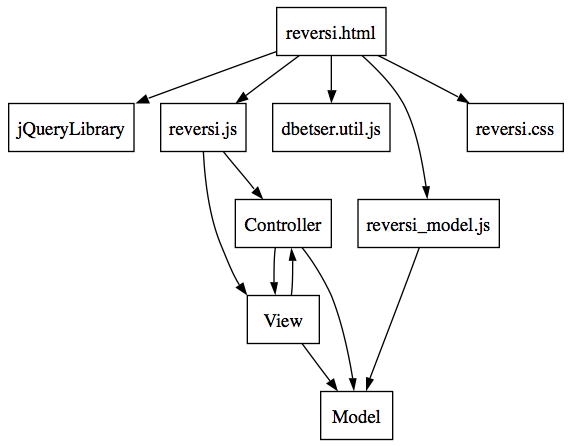
\includegraphics[width=350pt]{dot/moddepdiagram.png}
\label{fig:ob2} 
\end{center}
\subsection{Code Notes}
The most major hack that was included in the project deals with updating the player whose turn it is during undo/redo moves. One of the problems with my implementation was that for the two different types of play (versus computer and versus human), the current player during undo needed to be switched for versus human play and needed to stay the same for versus computer play. I included a hack to manually switch the current player in the \texttt{getCurrentBoardState} function based on the type of play. This allowed the current player to be correctly displayed even after a series of undos and redos.

Another note is regarding the representation of markers in the UI. In order to present a box's state, I wanted to be able to include a round circle representing the marker that would be used in a real Othello game. However, to do this, I needed to figure out how to change the CSS to include the image of the circle. Using CSS sprites seemed to do the trick for that.
\section{Testing}

\subsection{Test Plan}
To test the application, the HTML was validated to ensure standards compliance. Lint was run to avoid poor programming constructs.

The testing for this project was mostly manual. The below was done in both the Firefox and Chrome browsers.

I developed a number of test cases that ensured that the game functioned as specified.

\subsection{Test Cases}
To test the board itself, I did the following:
\begin{itemize}
\item Play the game until both players have won, in the versus computer and versus human modes. Ensure that the outcome message is displayed appropriately in all cases (black wins, white wins, tie).
\item Ensure that refreshing resets all state during any other time of game play.
\item Ensure that once a first box is selected, another box can be selected without affecting the model.
\item Test undo/redo with both modes to ensure that the board, statistics, and hovering marker change accordingly.
\item Test various combinations of undo/redo to ensure that no bug occurs when restoring state.
\end{itemize}

\subsection{Rationale and Conclusions}
This project fulfills the requirements of the assignment. The application runs as desired, and even implements undo/redo in a sophisticated and extensible way. Because I used extra slack days, I was able to debug to create a much cleaner and smoother product than I would have otherwise!

Many of the design decisions implemented made the interface easier and cleaner to use, which improved the overall user experience.

\end{document}

